\documentclass{article}
\usepackage[utf8]{inputenc}
\usepackage{amsmath}
\usepackage{listings}
\usepackage{geometry}
\usepackage{graphicx}
\usepackage{appendix}
\usepackage{subfig}
\usepackage{gensymb}
\usepackage{cancel}
\usepackage{physics}
\usepackage[colorlinks=true]{hyperref}
\usepackage{xcolor}
\definecolor{codegreen}{rgb}{0,0.6,0}
\definecolor{codegray}{rgb}{0.5,0.5,0.5}
\definecolor{codepurple}{rgb}{0.58,0,0.82}
\definecolor{backcolour}{rgb}{0.95,0.95,0.92}
\lstdefinestyle{mystyle}{
    backgroundcolor=\color{backcolour},   
    commentstyle=\color{codegreen},
    keywordstyle=\color{magenta},
    numberstyle=\tiny\color{codegray},
    stringstyle=\color{codepurple},
    basicstyle=\ttfamily\footnotesize,
    breakatwhitespace=false,         
    breaklines=true,                 
    captionpos=b,                    
    keepspaces=true,                 
    numbers=left,                    
    numbersep=5pt,                  
    showspaces=false,                
    showstringspaces=false,
    showtabs=false,                  
    tabsize=2
}

\lstset{style=mystyle}

\title{%
Project 1 - Studying a Bosonic Gas using a \\ Variational Monte Carlo method\\
\large FYS4411 at University of Oslo}
\author{Simen Løken}
\date{March 2023}
\footskip = 90pt
\topmargin = -40pt

\begin{document}
\nocite{*}
\maketitle
{
  \hypersetup{linkcolor=black}
  \tableofcontents
}
\newpage
\section{Abstract}
We examine various configurations of a Variational Monte Carlo system and find an optimal value for $a=0.5$. We then further explore methods to optimize our system by introducing sampling, resampling and a gradient descent method. The gradient descent method confirms what we found previously of $a=0.5$ being the optimal value. We find that in terms of sampling, importance sampling (although more computationally intensive) is superior to the more brute-force metropolis algorithm, especially as system complexity increases. 
\section{Introduction}
When one is studying quantum mechanical systems, it can often be hard to find exact analytical answers, and we must thus often make due with numerical solutions of varying complexity. A common and very popular method to use for studying such systems numerically is the Variational Monte Carlo method (henceforth VMC), which compared to its more complex many-body brethren often gives comparable results with a fraction of the effort, both in being numerically more lightweight and easier to implement.
\newline
It is therefore we intend to study and expand upon a VMC in this project, both to serve as an introduction to quantum mechanical systems and to study a Bosonic Gas. We will study the gas in multiple different configurations, including two different harmonic oscillators (one spherical and one elliptical), and with both interactive and non-interactive particles.
\section{Theory and Method}
\subsection{Monte Carlo and the Variational Monte Carlo} \label{mc}
The Monte Carlo is a well known method which uses randomized (and repeated) sampling to yield numerical results to various systems, but whereas the regular Monte Carlo method is more specialized in areas like integration, Variational Monte Carlo method is instead a variational method that approximates ground states of quantum systems. \newline
Assume we have some Hamiltonian $\mathcal{H}$ where the expecation value of the energy is given as:
\begin{equation*}
    E(a) = \frac{\langle \psi(a) \mathcal{H} \psi (a) \rangle}{\langle \psi (a) | \psi (a) \rangle}
\end{equation*}
where we assume $\psi$ to be some generic wave function that is dependent only on $a$. Thus, $a$ is our only variable which makes this a whole lot simpler. \newline
As we wish to find the ground state of the system, we must vary the variable $a$ so as to find the lowest possible energy $E$ of the system, thus giving us a better and better (as we approach the nominal analytical value of the system) numerical representation of the system. To do this, we're going to need to find the local energy $E_L$ and minimize it. The local energy can be expressed as:
\begin{equation} \label{linear}
    E_L(a) = N M a \frac{1-4a^2}{2} \sum_{n=1}^N r_n^2
\end{equation}
where $N$ is the number of particles in the system, $M$ is the dimension of the system and $r$ is the position of some particle $n$. To see the full derivation of this equation, see appendix $\ref{app1}$.
\subsection{Sampling}
The Variational Monte Carlo method relies on sampling to produce sufficient numerical results. We're going to be using two sampling methods for our calculations, the metropolis algorithm (which will henceforth be called the brute force method) and importance sampling. \newline
For the brute force method, we have some system of $N$ particles in an initial state. We then allow one of the particles to move at random, from some position $x_1$ to some position $x_2$. Whether or not we accept this move depends on the following condition:
\begin{equation}
    P \geq \frac{|\psi(r_j)|^2}{|\psi(r_i)|^2}
\end{equation}
where $P$ is a random value (or probability, if you will) selected for each move by a uniform distribution. \newline
Regardless of acceptance, we sample the energy level which we use to find the expectation value. \newline
Importance sampling is a more efficient method of solving our system numerically. Whereas the movements allowed for the particles were entirely random for the brute force method (hence brute force), with importance sampling we introduce a directional bias. Ultimately, we arrive at a force we name the drift force, or quantum force, which as the name suggests causes the particle to drift towards coordinates where the trial wave function is large. The force can be expressed as:
\begin{equation}
    \mathbf{F} = 2 \frac{1}{\psi_T} \nabla \psi_T
\end{equation}
and stems from the Fokker-Planck equation. The full derivation can be found at ref \cite{week3}.
\subsection{Gradient Descent}
We mentioned in \ref{mc} that we only aim to minimize one single variable to optimize our system, which leads us into the method we're going to be using to do this. Although we could probably "guesstimate" a pretty close variable $a$ that would get us close to the nominal value of the system, the best way to do this would be to automate the process so as to get as close as possible to the best representation of the system. We also mentioned that we wish to find the minima of the local energy $E_L$. The easiest way to do this is to use a gradient descent method. \newline
The gradient descent method aims to automatically find the minima from a given point along the "curve" of energy values given rise to from $a$. To do this, we select randomly an $a$ (preferably close to what we might think is the optimized value so as to save time) and calculate the derivative of the energy curve in that point. We then multiply our value $a$ by the gradient/derivative and some learning rate $\eta$. Once the "slope" of the gradient is sufficiently close to $0$, we retrieve the value $a$ and use it for further calculations. \newpage
\subsection{Data Analysis and resampling} \label{blo}
Although we could read the retrieved data "raw" without any further adjustments/touch ups, we could benefit from certain methods to further optimize our numerical data. The reason and motivation as to why we do this is because we're dealing with a system of i.i.ds (independent and identically distributed). Typically with systems such as these, the typical and most common ways of calculating errors tend to be a bit too gracious with our accuracy, and overestimates how accurate we actually are. In order to remedy this (somewhat), we're primarily going to be using two methods, bootstrapping and blocking. 
\newline Bootstrapping, which is best suited for smaller samples, intends to "mimic" the sampling process by randomly sampling with replacement. Assume we wish to do some measurement that is practically impossible in scope. Instead, we measure some small subset $N$ and measure it's mean to get a better understanding of the grander set of data. However, to get a better, broader understanding, we "shuffle" the subset $N$ and again sample the data. This over time, will generate a better mean and estimate of our grander data set.
\newline In mathematical terms, imagine we have some array $\mathcal{X}$ which contains $x_1, x_2, x_3 ... x_N$. We do our calculations on this set, then shuffle the data. Say we then end up with $x_2, x_2, x_5, ... x_N$. Assuming $\mathcal{X}$ is sufficiently large, shuffled $\mathcal{X}$s will never be the same and we can thus get "more value" out of a small subset of data.
\newline
As opposed to bootstrapping, blocking is more suited for larger data sets. This is, in part, because unlike bootstrapping where the resampling a some data of size $N$ retains its size, with blocking we reduce the size of the data set through the process. For a dataset of size $2^N$, blocking aims to take the average of neighbouring data points in a vector to replace values. This in turn means that for each blocking iteration we halve our dataset, resulting in $2^{N-1}$ all the way until we have only one value left. This is an estimate of the mean of the dataset.
\subsection{Our System}
Let us last discuss our system and how we're going to proceed. We're going to, as discussed, examine many various configurations and methods to calculate our numerical results. To aid in better illustrating this, let us assume we have some system we wish to examine with $N$ particles and $M$ dimensions. We initialize the system, evenly distributing the different particles using a normal distribution. From there, we start iterating. For each iteration in our VMC algorithm, we're going to be going through each particles and moving it some distance, again decided at random. After each move, we're going to extract values (energy, wave function value). We can then store these values and use them for our numerical calculation. In very simple pseudo-code, we end up with:
\begin{lstlisting}[language=Python]
for i in itrs:
    for j in N:
        particle[j].move()

        system.getEnergy()
        system.getWaveFunction()
    
\end{lstlisting}
To keep it neat and tidy, we're going to be using classes to keep the system as modular as possible
\section{Results}
We run initial tests to check local energy $E_L$ of a one-dimensional system against different values of $a$:
\begin{figure}[ht!]
    \centering
    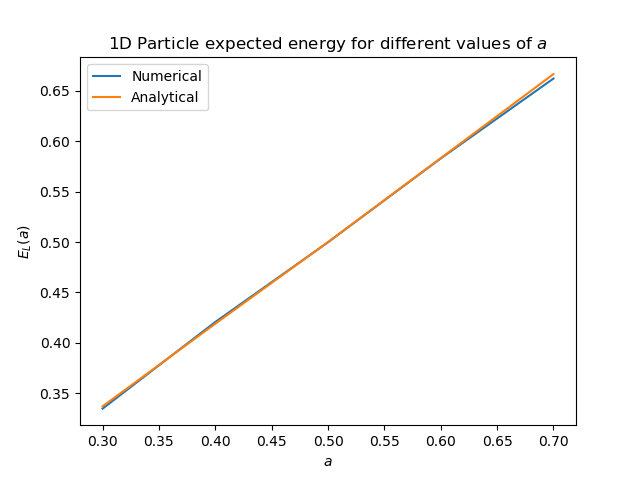
\includegraphics[scale=0.4]{fig_b1.png}
    \caption{An analytical solution for different values of $a$ vs a numerical one. \newline
    As this was done with just one particle in one dimension, there is little to no deviation from the analytical solution. \newline Were we to increase the complexity either through increasing the dimensionality or the number of particles, the numerical solution would deviate more and more from the analytical. This suggests that the brute force method is more suited to simple VMC systems.}
    \label{fig:my_label}
\end{figure} \newline
We see here quite clearly that $a = 0.5$ remains the best and most accurate to the analytical solution. We see also that the numerical solution is very, very close to the analytical one for a single one-dimensional particle.
\begin{figure}[ht!]
    \centering
    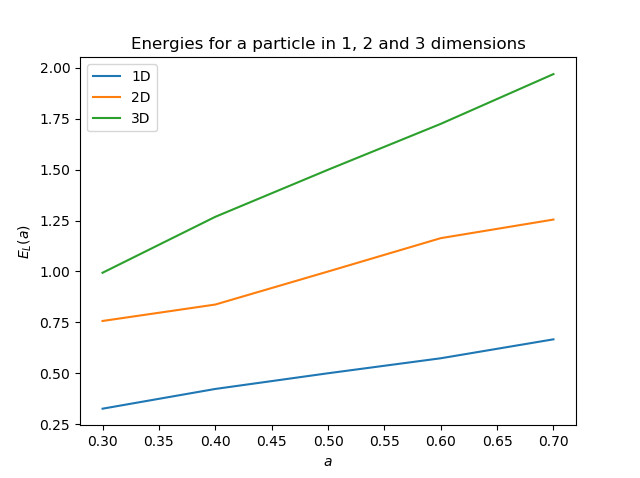
\includegraphics[scale=0.4]{fig_b2.png}
    \caption{We see here a direct linear correlation in relation to the dimensionality of the system, as expected from \ref{linear}}
    \label{fig2}
\end{figure} \newline
Here we can see that the energy levels of the system have a direct linear correlation with the dimensions of the system. This isn't so odd when you consider the equation \ref{linear}, which as we can see scales linearly with both dimension and number of particles. To double-check this, we can plot for different numbers of particles and then divide the final energy by the number:
\begin{figure}[ht!]
    \centering
    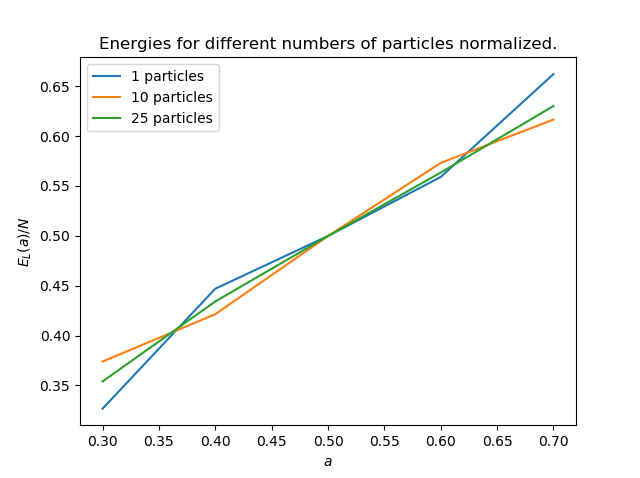
\includegraphics[scale=0.4]{fig_b3.png}
    \caption{We see here clearly the linearity as we increase the number of particles in the system.}
    \label{fig3}
\end{figure} \newline
Let us now examine the ways we previously discussed of optimizing our results. First, let us make sure that the value $a$ we found is actually the optimal one. For this we use the gradient descent method, and find:
\begin{figure}[ht!]
    \centering
    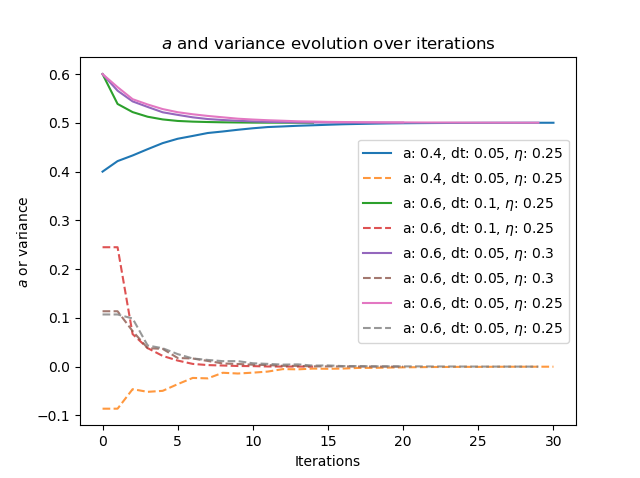
\includegraphics[scale=0.4]{fig_d1.png}
    \caption{A figure showing how variance and $a$ converge over different numbers of iterations for different configurations. The variance converges to 0 as expected and the value $a$ converges to $0.5$. \newline
    This could perhaps be made more efficient with a modular learning rate as opposed to a static one, although it is not a big issue. \newline
    The calculations were done with 100 particles in 3 dimensions, without importance sampling}
    \label{fig:my_label}
\end{figure} \newline
We see here that every initial condition gravitates towards a value $a=0.5$ as was expected.\newpage
Let us now examine how our numerical calculations can be improved using importance sampling instead of the brute-force method:
\begin{table}[ht!]
    \centering
    \begin{tabular}{cccccccc}
         a& & Brute Force& & & & Importance Sampling& \\
         \hline \hline
         & \left|\psi\right|^2 & E_L & \sigma & \vline&\left|\psi\right|^2 & E_L & \sigma & \\
         \hline
         0.3&  0.916& 10.49& 38.09& \vline& 0.941& 9.718& 1.528& \\
         0.4& 0.779& 12.95& 31.73& \vline& 0.927& 12.48& 1.952&\\
         0.5& 0.837& 14.99& 1.952& \vline& 0.947& 14.99& 0.063&\\
         0.6& 0.793& 16.89& 41.19& \vline& 0.84& 17.56& 1.617&\\
         0.7& 0.857& 18.63& 64.23& \vline& 0.82& 19.66& 1.54&
         \hline
    \end{tabular}
    \caption{We see here the values of $|\psi|^2$, $E_L$ and $\sigma$ compared across two different methods of sampling. As this was done for "medium"-level system complexity, we confirm what we thought that importance sampling is more suited as the system complexity increases, whereas brute-force only really does well in very simple system. \newline
    Take note that this does not mean brute-force performs better than importance sampling in simple systems, but it is computationally less expensive than importance sampling.}
    \label{tab:my_label}
\end{table} \newline
We see here that importance sampling is much more efficient in terms of error and accuracy than it's brute-force counterpart, as is to be expected. However, as discussed in \ref{blo} these accuracy measurements can be overly optimistic, and we can instead apply resampling techniques to better gauge the error of our system. \newline
We examine bootstrap with a total of 250 resamplings and compare it to importance sampling:
\begin{table}[ht!]
    \centering
    \begin{tabular}{ccc}
         a& Importance [\sigma]& Bootstrap_{250} [\sigma]&  \\
         \hline
         0.3& 1.528& 3\times 10^{-4}& \\
         0.4& 1.952& 2\times 10^{-4}& \\
         0.5& 0.063& 9\times10^{-9}& \\
         0.6& 1.617& 2\times 10^{-4}& \\
         0.7& 1.54& 5\times 10^{-4}&
         \hline
    \end{tabular}
    \caption{We see here the errors from the previous table compared with the errors brought forth from using a bootstrap method with 250 resamplings.
    Take note that this is opposite of what we expected to get (ie. the bootstrap method should return greater errors than its non-bootstrapped counterpart), which suggests something is wrong with one of the error-estimations.}
    \label{tab:my_label}
\end{table} \newline
We see here that we get a much, much lower estimate of the system error, somewhat surprisingly. \newpage
\section{Discussion}
\subsection{Further discussion of results}
I'll now address the "elephant in the room", so to speak. The interactive model is missing. For various reasons I ultimately did not have time to implement it outside of the potential energy of the system now accounting for the potential being infinite when $r \leq a$. However, I do believe that the only thing (and it is admittedly a pretty big thing) missing was a way to calculate the laplacian for the interactive system. Once this had been done, I'm fairly certain we would've atleast had some results to examine, ableit perhaps unoptimized and underdeveloped.
\newline
As for the other results, I'm fairly certain something went wrong with the bootstrap method. To my understanding, resampling methods should increase the error because, as discussed, in cases where we're dealing with i.i.d the error estimation tends to be a bit optimistic. It is of course also possible that the bootstrap method is actually correct and that my other error estimation (using variance from energy) is incorrect. \newline
The other results I did get I am fairly happy with. With figures like \ref{fig2} and \ref{fig3}, where one of my goals was to show the linearity of the energy $E_L$ with respect to both dimensional spacing and number of particles, I could've probably done multiple runs and then plotted the average of those runs so as to better illustrate that they truly are linear. Ultimately I did not find the time for this, but I do think most of the other results are inline with reality and not far off what they should be.
\subsection{The choice of time step}
Initially, for much of my initial exploration of the system, I was operating with a static timestep of $\delta t = 1\times10^{-4}$. Although this led to very nice results, I had an issue where it cause the variance, calculated by:
\begin{equation*}
    var = \sum_{i=0}^N E_i^2 - \left(\sum_{i=0}^N E_i \right)^2
\end{equation*}
to always be zero, thus making a gradient descent method (where we look for a value $a$ that minimizes the variance) seemingly impossible. Letting then $\delta t$ be bigger got us actual results which meant we were able to numerically find an optimal value for $a$. \newline
In retrospect, it might have also been caused by initially testing on a numerically small system (few particles, low number of dimensions). Regardless, I decided to for most of the calculations to operate with a $\delta t = 0.01$.
\subsection{Parallelizing the program}
Although (seemingly(?)) very trivial to parallelize, I ran into some issues where it wouldn't actually cause any noticable speed up. Instead, it caused noticable slowdown, often in the magnitude of $10$x the single threaded run speed. Initially I suspected it to be caused by the built in python function \texttt{copy.deepcopy()} which I used to make copies of the system multiple times. Ultimately, even with functionality removed the issues with parallel being slower persisted, and wound up spending way too much time trying to fix it, which is partially why the interactive case is only partially implemented. I know that certain python libraries do use parallelization natively and, although unlikely, it is perhaps possible that this with the multi-threaded process somehow caused the computation to "hang". Ultimately I do not know why this slowdown was so severe.
\section{Conclusion}
In this report we've looked at how to setup and optimize a variational monte carlo algorithm to study a quantum mechanical system of various shapes and sizes. We've produced various results, finding the value $a=0.5$ to be most efficient when wishing to study these systems numerically. We then double checked this using a gradient descent method, and found an agreeable value $a$. We've also in length discussed and showed various sampling methods for our VMC and how these can lead to better results.
\bibliographystyle{plainurl}
\bibliography{citations.bib}
\newpage
\renewcommand*\appendixpagename{\Large Appendices}
\appendixpage
\addappheadtotoc
\renewcommand{\thesubsection}{\Alph{subsection}}
\subsection{Finding expressions} \label{app1}
We were asked to find some expressions in $1a)$.
\newline
We have first the initial trial wave function:
\begin{equation*}
    \psi_T (r) = \left[ \prod_i g(\alpha, \beta, r_i \right] \left[ \prod_{j<k} f(a|r_j - r_k) \right]
\end{equation*}
which we may simplify as:
\begin{equation*}
    \psi_T (r) = \prod_i g(r_i) \exp \left(\sum_{i<j} u(r_{ij}) \right)
\end{equation*}
We now need both the first and the second derivative of this. We start by finding the first derivative as:
\begin{equation*}
    \nabla_k \psi_T (r_k) = \nabla_k g(r_k) \left[ \prod_{i\neq k} g(r) \right] \exp \left( \sum_{i<j}^N u(r_{ij}) \right) + \left[\prod_i^N g(r_i) \right] \exp \left( \sum_{i<j}^N u(r_{ij}) \right)  \sum_{i \neq k}^N \nabla_k u(r_{ik})
\end{equation*}
Thus we need to find:
\begin{equation*}
    \frac{1}{\psi_T (r)} \nabla_k \nabla_k \psi_T (r)
\end{equation*}
which, through much tedious deriviation and calculation, becomes:
\begin{equation}
\boxed{
\begin{split} 
    \frac{1}{\psi_T (r)} \nabla_k \nabla_k \psi_T(r) = \frac{\nabla_k^2 g(r_k)}{g(r_k)} + 2 \frac{\nabla_k g(r_k)}{g(r_k)} \sum_{j\neq k} \frac{r_j - r_k}{r_{jk}} u'(r_{jk}) + \\ \sum_{i\neq k} \sum_{j\neq k} \frac{(r_k - r_i)(r_k - r_j)}{r_{ki} r_{kj}} u'(r_{ki}) u'(r_kj) + \sum_{j\neq k} \left( u''(r_{kj} + \frac{2u'(r_{kj}}{r_{kj}}\right)
\end{split}}
\end{equation}
\subsection{Runtimes}
We were additionally asked to compare runtimes and how differing variables and setups had an effect. I found no logical place to put this in the actual report so I leave it here to the appendix. \newline
Both ways in which we increase complexity (particles and dimensionality) leads to an exponential growth in computation time. Just going from $N=1$ to $N=5$ is a $9$x increase of baseline computation time, whereas going from $N=1$ to $N=10$ is a $47$x, in just a single dimenion. If we instead increase dimensionality, we find that $1\times3$ to $5\times 3$ is a $21$x increase and going all the way to $10\times 3$ is a $123$x increase in computation time. \newline 
I mentioned at various times that importance sampling is more computationally intensive than the brute force metropolis algorithm. \newline
Ultimately, in terms of performance there is a lot of leeway for improvement. Both in terms of going from Python to a faster language like c++, or cutting out unnecessary calculations where they are unneeded. \newpage For this project, I focused less on faster run times and optimization and more on making it as modular and usable (and re-usable) as possible as my Master's Thesis will involve using such a method and this project (and the code developed) serves as a good starting point to branch out from and to study further.
\subsection{Code + more}
Code and data, figures and raw latex can be found at: \newline \href{https://github.com/simloken/FYS4411/tree/master/Project_1}{\texttt{https://github.com/simloken/FYS4411/tree/master/Project\textunderscore1}}
\end{document}
